\documentclass[11pt]{article}
\usepackage{fontspec}
\setmainfont{NotoSerif-Regular.ttf}[Path=C:/Windows/Fonts/,ItalicFont=NotoSerif-Italic.ttf,BoldFont=NotoSerif-Bold.ttf,BoldItalicFont=NotoSerif-BoldItalic.ttf]
\usepackage[a4paper,margin=22mm]{geometry}
\usepackage{amsmath,amssymb,graphicx,xcolor,hyperref,needspace}
\usepackage[normalem]{ulem}
\let\MathUnderline\underline
\renewcommand{\underline}[1]{\ifmmode\MathUnderline{#1}\else\uline{#1}\fi}
\hypersetup{unicode=true,colorlinks=true,linkcolor=blue,pdfauthor={}}
\setlength{\parindent}{0pt}
\setlength{\parskip}{.4em}
\setlength{\emergencystretch}{3em}
\raggedright
\newcommand{\SourcePage}[2]{\par\smallskip\phantomsection\label{#1:source-page}{\small\sffamily\color{blue!55!black}#1}\par\smallskip}
\newcommand{\EvidenceBlock}[4]{%
 \par\smallskip\noindent\begin{minipage}{\linewidth}
 \begin{minipage}[t]{.47\linewidth}\vspace{0pt}\centering
 \csname evidence-#1-#2\endcsname\par
 {\scriptsize\SourceCropCaption\ #1}\par
 \end{minipage}\hfill
 \begin{minipage}[t]{.49\linewidth}\vspace{0pt}\raggedright
 {\small\color{orange!65!black}\textbf{#4} #3}\par
 \end{minipage}
 \end{minipage}\par\smallskip}
\newcommand{\Unclear}[3]{\EvidenceBlock{#1}{#2}{#3}{\ReadingCaption}}
\newcommand{\Incomplete}[3]{\EvidenceBlock{#1}{#2}{#3}{\IncompleteCaption}}
\newcommand{\SourceFigure}[3]{\EvidenceBlock{#1}{#2}{#3}{\DiagramCaption}}
\expandafter\def\csname evidence-GELFAND-P000001-module-letter\endcsname{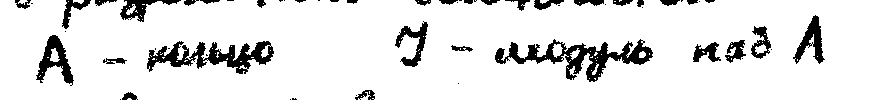
\includegraphics[width=\linewidth]{figures/gelfand-p000001-module-letter-original.png}}
\expandafter\def\csname evidence-GELFAND-P000001-diagram-blowup\endcsname{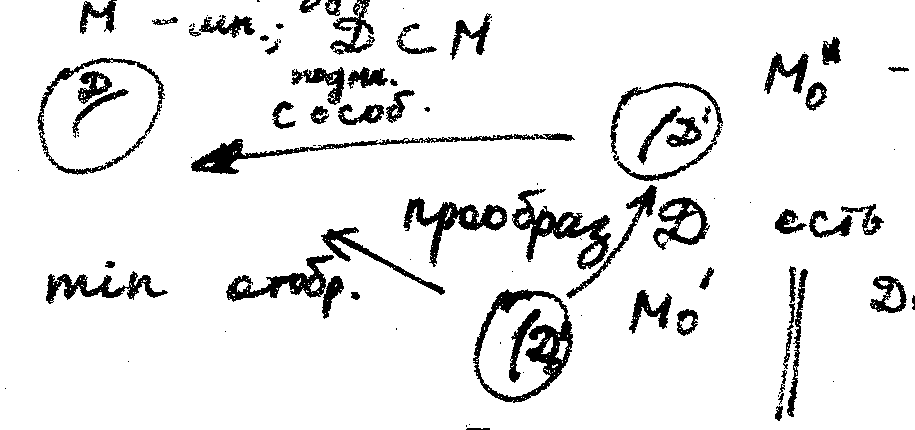
\includegraphics[width=\linewidth]{figures/gelfand-p000001-diagram-blowup-original.png}}
\expandafter\def\csname evidence-GELFAND-P000001-blowup-notation\endcsname{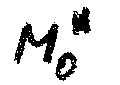
\includegraphics[width=.43\linewidth]{figures/gelfand-p000001-upper-blowup-label-original.png}\hfill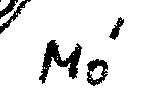
\includegraphics[width=.50\linewidth]{figures/gelfand-p000001-lower-blowup-label-original.png}}
\expandafter\def\csname evidence-GELFAND-P000001-origin-example\endcsname{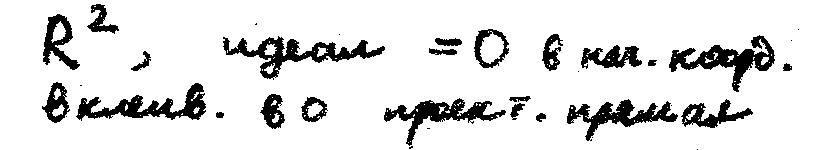
\includegraphics[width=\linewidth]{figures/gelfand-p000001-origin-example-original.png}}
\newcommand{\SourceCropCaption}{Original source details:}\newcommand{\ReadingCaption}{Uncertain reading.}\newcommand{\IncompleteCaption}{Undeciphered passage.}\newcommand{\DiagramCaption}{Diagram and typed description.}
\hypersetup{pdftitle={Gelfand seminar — chapter 1}}
\begin{document}
{\large\bfseries Gelfand seminar — chapter 1}\par
{\small Opening of the reader. Source frame 1. Text and formulas are typed; original details accompany every uncertain reading. Working excerpt; the complete chapter is still in preparation.}\par\medskip
\SourcePage{GELFAND-P000001}{unlabelled}
Monday, $21/\mathrm{IX}$.
Cartesian and Boolean products of groups.

``Hironaka: on resolution of singularities.''
\underline{Gelfand}

$A$ is a ring, $\mathcal{J}$ is a module over $A$.
\Unclear{GELFAND-P000001}{module-letter}{The letter for the module and ideal is rendered as $\mathcal{J}$; $\mathcal{I}$ or $J$ are possible.}

Blow-up --- ?
$M$ is a manifold; $D\subset M$.
[Beneath $D$:] a subset with singularities.

$M_0^H$ is the blow-up. Blowing-up.
The inverse image of $D$ is $D'$, a manifold of dimension $n-1$.
$D_0$ is $(n-1)$-dimensional.
\SourceFigure{GELFAND-P000001}{diagram-blowup}{Three enclosed drawings: at left a region with $D$; at upper right a region with $D'$ and the label $M_0^H$; at lower right a region and the label $M'_0$. The upper arrow points left; the lower oblique arrow also points left, with the label ``continuous map'' [source abbreviation: непр. отобр.]. The precise inner curves, labels and the connection of the lower region to the upper one require comparison with the scan.}
\Unclear{GELFAND-P000001}{blowup-notation}{The upper index on $M_0$ resembles $H$; the lower region's label resembles $M'_0$.}

The construction is Grothendieck's.
$A$ is a ring, $\mathcal{J}$ is a module.
\underline{Example.} $A$ is a ring of functions;
$\mathcal{J}$ is the ideal of functions taking the value $0$ on $D$.

One obtains a sheaf of rings and a sheaf of modules.
$A$ is a ring, $\mathcal{J}$ is an ideal.
Construct $X$, $O_X$ a sheaf of rings,
$\mathcal{J}_X$ a sheaf of ideals, so that
\begin{gather*}
 (A,\mathcal{J})\ \longleftarrow\ (X,O_X,\mathcal{J}_X).
\end{gather*}
[Beneath the arrow:] linear map.

$(A,\mathcal{J})$ is a sheaf generated by $1$ ideal.

$\mathcal{J}_X$ is invertible, i.e. an ideal of the ring:
$\exists f\in\mathcal{J}_X$ such that $O_Xf=\mathcal{J}_X$.
[Above the formula, an arrow to $\exists$:] generator.

(The ideal is principal if $\mathcal{J}$ is an ideal.)
Then the zero variety is $1$ equation.

$A$ is a ring, $\mathcal{J}$ is an ideal.
\underline{Typical example:} $R^2$, the ideal $=0$ at the origin.
\Unclear{GELFAND-P000001}{origin-example}{The next line: ``Gluing a projective line into $0$'' [source: Вклеив. в $0$ проект. прямой]; the beginning may read ``Оклеив.''.}

$A$, $\mathcal{J}$ are modules.
\begin{gather*}
 \mathcal{J}\otimes_A\mathcal{J},\qquad
 \mathcal{J}\otimes_A\mathcal{J}\otimes_A\mathcal{J},\ldots
\end{gather*}
[Above the groups of tensor products:] symmetric; symmetric.

Consider formal sums
\begin{gather*}
 \sum_{k=0}^{N}a_kz^k.
\end{gather*}
Add and multiply.
$x\otimes y=y\otimes x$.
\begin{gather*}
 a_0\in A,\qquad a_1\in\mathcal{J},\qquad
 a_2\in\mathcal{J}\otimes_A\mathcal{J}\quad\text{—}
\end{gather*}



\clearpage\section*{Full reading notes}
\subsection*{GELFAND-0001-U001}
\EvidenceBlock{GELFAND-P000001}{module-letter}{After “A is a ring” is a handwritten letter with a fork at the top and a lower hook; it recurs for the module and the ideal.}{Observation.}
\textbf{Candidates: } \(\mathcal{J}\); \(\mathcal{I}\); J\par
\textbf{Historical note: } A calligraphic J was used in the text as a graphical candidate; the notation was not identified from its mathematical meaning.\par
\textbf{Fresh source comparison: } The same fork and lower hook are visible in three separate occurrences at 5×/10×. This supports a consistent graphical transcription but does not distinguish every possible conventional I/J letterform.\par
\subsection*{GELFAND-0001-U002}
\EvidenceBlock{GELFAND-P000001}{diagram-blowup}{In the upper half are three rounded contours with inner curves and two leftward arrows; D,D-prime,M and indices occur above and beside them.}{Observation.}
\textbf{Candidates: } None proposed.\par
\textbf{Historical note: } Uncertain inner curves and joins were not redrawn. The description and the source-figure entry retain a locator for comparison.\par
\textbf{Fresh source comparison: } The complete diagram crop is now displayed at its typed description. Both leftward arrowheads are visible. A separate curved stroke rises from the lower contour toward the area beside D; its exact attachment to the upper contour is not asserted.\par
\subsection*{GELFAND-0001-U003}
\EvidenceBlock{GELFAND-P000001}{blowup-notation}{The upper index on \(M_0\) resembles H; over \(M_0\) at the lower region is a short stroke.}{Observation.}
\textbf{Candidates: } \(M_0^H\); \(M'_0\); \(M_0^N\); \(M'_0\)\par
\textbf{Historical note: } The indices and prime need comparison with the original.\par
\textbf{Fresh source comparison: } Separate close crops show the dark upper index and the lower prime at the reading itself. The lower prime is distinct; the dark upper sign still does not justify excluding N in favor of H.\par
\subsection*{GELFAND-0001-U006}
\EvidenceBlock{GELFAND-P000001}{origin-example}{To the right of the \(R^2\) example the line begins with a joined group of letters and ends “into 0,a projective line”.}{Observation.}
\textbf{Candidates: } Вклеив. в 0 проект. прямой [Gluing a projective line into 0]; Оклеив. в 0 проект. прямой [alternative initial abbreviation]\par
\textbf{Historical note: } The phrase is given inside the uncertain-reading entry,without choosing from the mathematical meaning of a blow-up.\par
\textbf{Fresh source comparison: } The wider context and 5×/10× details strongly favor the initial В and the abbreviation Вклеив. The historical alternative remains visible; the source wording is not replaced by a standard construction of a blow-up.\par
\end{document}
